\section{Camera Module Testing - (mh)}

The camera module and controller were tested throughout their development and thus problems were quickly discovered and swiftly rectified.

\subsection{Test: uCam Existing Software (jc)}
\label{sec:existing_software_test}

The uCam has a freely downloadable piece of software (downloadable from \cite{ucam_test_software}) that allows you to test the uCam and verify its functions. If you can connect the uCam to a COM port on the computer then you can sync with it and then take and view pictures in the different available formats and resolutions.

This allowed for not just the functionality of the camera to be verified but said functionality was then compared to the specification and it was shown that the uCam should be able to provide what is required from the camera module.

The uCam was connected to a host PC using a USB to Serial cable and tested using the software. The software connected to the camera successfully and downloaded an image as expected.

This task did not verify any milestones, but it did show clearly that the camera was working. In the event of the camera becoming unresponsive, this software helped us diagnose the problem, since if the camera worked with this software it was clearly a problem with our implementation, while if the camera did not work with this software then it would suggest the camera itself was at fault. Before declaring any of the cameras used in the project faulty they were checked using this software.

\subsection{Test: Basic Connection Test on Arduino (mh)}
\label{sec:basic_connection_test}

The first step when communicating with the camera module is to establish a connection to it.  The implementation code follows the procedure shown in figure \ref{fig:syncProto} to connect to the camera, sending SYNC commands until the appropriate response is detected from the camera, indicating a successful connection and so the success of this test.

\begin{figure}[H]
        \centering
        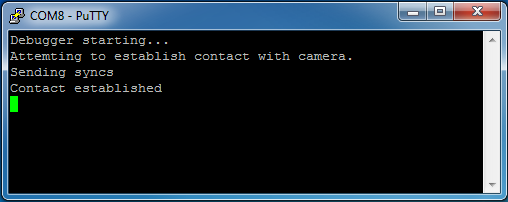
\includegraphics[width=1.0\textwidth]{testing_screenshots/camera_basic_connection_test.png}
        \captionof{figure}{Testing our implementation of the basic connection to the camera module.}
        \label{fig:test_basic_connection}
\end{figure}

Figure \ref{fig:test_basic_connection} shows the result of a test for basic connection to the camera module. In figure \ref{fig:test_basic_connection} the line ``Contact established'' means the Arduino has detected these correct responses. With this successful connection, milestone \ref{sec:ms_basic_cam_comm} is validated, meaning the implementation was free to move on.

\subsection{Test: Image from Camera - (mh)}
\label{sec:image_capture_test}

The first attempt at a simple test for this was to use the debug connection to the Arduino camera controller implementing the camera connection code to relay image data to a PC, unfortunately as described in section \ref{sec:misc_cam_probs} initial implementations of this were not successful, since the debug connection was not completely error free, causing the image to be malformed and unreadable.

However, at this point in the implementation the basic SD card communication had already been implemented as described in section \ref{sec:SD_imp}. Because of this, it was decided  that a much more sensible test would be to write the image data directly to the SD card. The test comprises of running the camera connection code on the microcontroller with the camera and SD card attached. Figure \ref{fig:test_camera_image_saving_sd_card} shows the debug information sent from the controller during this test and \ref{fig:Nyan1} shows the image saved to the SD card. The debug information suggests that the connection and download of image data was successful and the image on the SD card verifies this.

\begin{figure}[H]
        \centering
        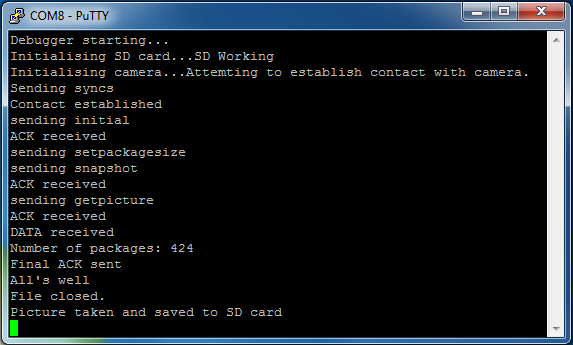
\includegraphics[width=1.00\textwidth]{testing_screenshots/camera_image_saving_sd_card_test.png}
        \captionof{figure}{Debug information sent from camera controller to PC while taking a picture and saving it to an SD card.}
        \label{fig:test_camera_image_saving_sd_card}
\end{figure}

\begin{figure}[H]
        \centering
        \includegraphics[width=1.00\textwidth]{figures/nyanNyan.jpg}
        \captionof{figure}{Test image captured using the Arduino implementation of the camera controller}
        \label{fig:Nyan1}
\end{figure}

The testing during development means that functionality of the controller has been verified already, the test that needs to be performed on this element of the system is to time how long it takes to get an image from the camera and save it to the SD-card and check that this is well within the 3 minutes allowed by the specification. Timing of this process showed that it took around 5 seconds to complete, so well within the 3 minute limit in the specification.

This test verifies milestone \ref{sec:ms_img_from_cam}. The resolution of the image is 640x480.

\subsection{Test: Change Resolution - (mh)}
\label{sec:test_change_resolution}

Since the option to change resolution was a low priority task it was implemented and tested after the basic main system - including image transmission over the autopilot link - was operational.

This test involved sending a Change Camera Resolution command to the payload module over the autopilot link from the ground station, checking the debug line for the correct response and viewing the images downloaded from the camera to verify resolutions.

\begin{figure}[H]
        \centering
        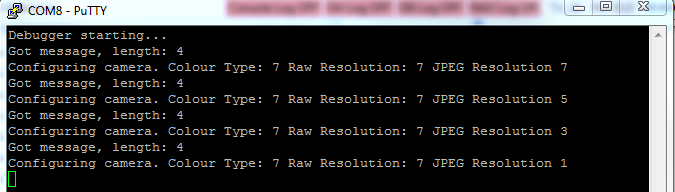
\includegraphics[width=1.00\textwidth]{testing_screenshots/change_res_debug_1.png}
        \captionof{figure}{Test images captured using the integrated implementation of the camera controller}
        \label{fig:test_change_res_debug_1}
\end{figure}

Figure \ref{fig:test_change_res_debug_1} shows the debug information sent from the payload module, the four ``Configuring Camera'' messages in the figure correspond to resolution change messages sent from the ground station. The resolution was changed to the four JPEG resolution values available one after another: 
\begin{itemize}
	\item \textbf{640 x 480}  - Corresponds to ``JPEG Resolution 7''
	\item \textbf{320 x 240} - Corresponds to ``JPEG Resolution 5''
	\item \textbf{160 x 128} - Corresponds to ``JPEG Resolution 3''
	\item \textbf{80 x 64} - Corresponds to ``JPEG Resolution 1''
\end{itemize}

The presence of the debug information recieved from the payload does not validate anything alone, therefore an image was taken at each resolution, shown in figure \ref{fig:change_res_debug}.

This test validates milestones \ref{sec:ms_img_cam_change_res} and \ref{sec:ms_pl_img_gs_cam_res}.

\begin{figure}[H]
  \centering
  \begin{tabular}{c c}
  \subfigure[640 x 480]{\label{fig:whole_fft_lfc}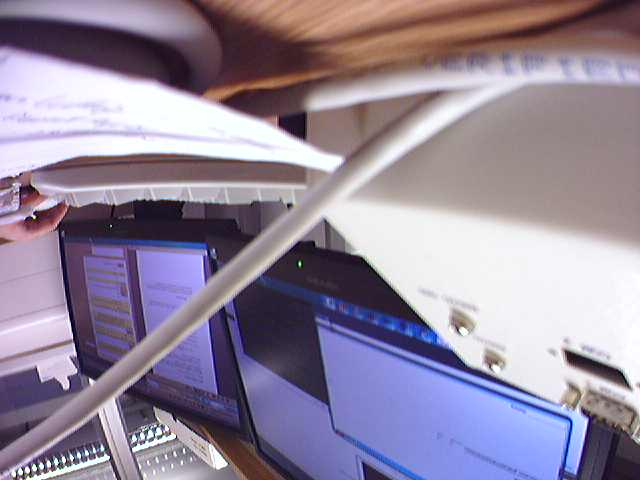
\includegraphics[width=0.5\textwidth]{testing_screenshots/res_pic_640_480.jpg}}&                
  \subfigure[320 x 240]{\label{fig:whole_fft_mfc}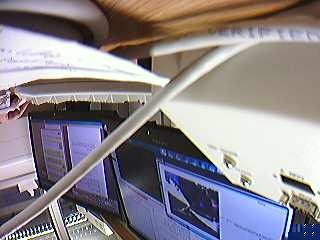
\includegraphics[width=0.25\textwidth]{testing_screenshots/res_pic_320_240.jpg}} \\
  \subfigure[160 x 128]{\label{fig:whole_fft_all}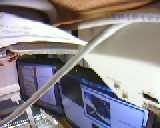
\includegraphics[width=0.125\textwidth]{testing_screenshots/res_pic_160_128.jpg}} &
  \subfigure[80 x 64]{\label{fig:whole_fft_all}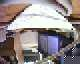
\includegraphics[width=0.0625\textwidth]{testing_screenshots/res_pic_80_64.jpg}}
  \end{tabular}
  \captionof{figure}{Images taken at various resolutions - these were saved by the ground station software after they were downloaded over the autopilot link.}
  \label{fig:change_res_debug}
\end{figure}



%\subsection{Final Camera Testing - (jc)}
%\label{sec:camera_integration_test}

%During the integration process the system was regularly tested for functionality and any errors were fixed as the system was developed. A large number of images were taken during this process and during the implementation of additional features.

%\begin{figure}[H]
    %    \centering
       % 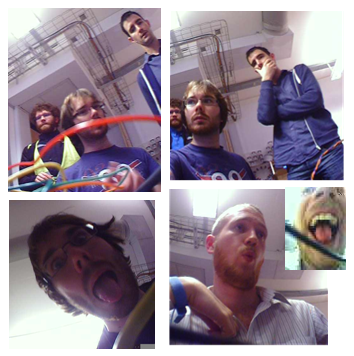
\includegraphics[width=1.00\textwidth]{figures/SampleImages1.png}
       % \captionof{figure}{Test images captured using the integrated implementation of the camera controller}
       % \label{fig:Samples1}
%\end{figure}

%The system can capture images at the 640x480 resolution specified and can also capture images at the other resolutions at which the uCam will take jpeg images. %Currently the option to capture raw images is not implemented.

%The time taken for the system to capture an image at maximum resolution, save it to SD-card and then download and display it on the ground station software was measured at 19.1s |||||||||REF|||||||||. This is still well within the 3 minutes specified and has large amounts of overhead meaning that it should remain well within that limit even if there are+ other payloads implemented on the UAV or if a lot of packets are dropped and have to be resent.

